\documentclass[a4paper, amsfonts, amssymb, amsmath, reprint, showkeys, nofootinbib, twoside]{revtex4-1}
\usepackage[english]{babel}
\usepackage[utf8]{inputenc}
\usepackage[colorinlistoftodos, color=green!40, prependcaption]{todonotes}
\usepackage{amsthm}
\usepackage{mathtools}
\usepackage{physics}
\usepackage{xcolor}
\usepackage{graphicx}
\usepackage[left=23mm,right=13mm,top=35mm,columnsep=15pt]{geometry} 
\usepackage{adjustbox}
\usepackage{placeins}
\usepackage[T1]{fontenc}
\usepackage{lipsum}
\usepackage{csquotes}

% for footnotes in tables
\usepackage{booktabs,caption}
\usepackage[flushleft]{threeparttable}

% for printing of units
\usepackage{siunitx}
\sisetup{load-configurations = abbreviations}

\usepackage{tikz}

% biblatex for references
\usepackage[sorting=none]{biblatex}
\addbibresource{Refer.bib}

% degree sign
\usepackage{gensymb}

% angstrom
\newcommand{\angstrom}{\mbox{\normalfont\AA}}




\usepackage[pdftex, pdftitle={Article}, pdfauthor={Author}]{hyperref} % For hyperlinks in the PDF
%\setlength{\marginparwidth}{2.5cm}
\bibliographystyle{apsrev4-1}
\begin{document}
\title{Laser shock peening acoustic emission measurement by evaluation of acoustic wave propagating through air}
\author{\textbf{Marek Böhm}\textsuperscript{1,2}, \textbf{Sunil Pathak}\textsuperscript{1},\textbf{Jan Kaufman}\textsuperscript{1}, \textbf{Jan Šmaus}\textsuperscript{1}, \textbf{Ondřej Stránský}\textsuperscript{3}}


% \date{\today} % Leave empty to omit a date

    %%%%%%%%%%%%%%%%%%%%%%%%%%%%%%%%%%%%%%%%%%%%%%%%%%%%%%%%%%%%%%%%%
    %%%%%%%%%%%%%%%%%%%%%%%%%%%%%%%%%%%%%%%%%%%%%%%%%%%%%%%%%%%%%%%%%
    %%%%%%%%%%%%%%%%%%%%%%%%%%%%%%%%%%%%%%%%%%%%%%%%%%%%%%%%%%%%%%%%%
    % ABSTRACT

\begin{abstract}
Acoustic emission (AE) monitoring is a non-destructive evaluation technique widely used to detect and analyse the acoustic waves generated by material deformation and damage. In this study, we applied AE monitoring to laser shock peening (LSP). We conducted LSP experiments on AA2024 samples and simultaneously recorded the AE signals generated during the process. The AE signals were analysed to identify the acoustic event of laser-induced breakdown in water. The results show that AE monitoring can provide valuable information on the LSP process and its effects on the material properties. Furthermore, the AE signals can be used to optimise the LSP parameters, such as the laser energy and spot size, to achieve the desired compressive residual stresses and avoid undesired damage. Overall, this study demonstrates the potential of AE monitoring as a tool for the in-situ characterisation of LSP, providing insights into the underlying physical processes and helping to improve the quality and reliability of the treated materials.
\end{abstract}

\keywords{laser shock peening, acoustic emission method, optical microphone, laser-induced breakdown}


\maketitle

\section{Introduction} \label{sec:outline}
    % Residual stresses evaluation based on acoustic signature of LSP

\subsection{Laser shock peening}

The configuration of an LSP process with a metallic component is shown in Figure~ \ref{fig:lspconfiguration}. An intense pulsed laser shock beam is focused onto a metal surface for a brief period of time (\SIrange{10}{100}{\ns}). The heated zone is vaporised and transformed to plasma by ionization (the temperature of plasma is over \SI{10000}{\degreeCelsius}). The plasma is under high pressure, which propagates through the material via shock waves. Two modes of LSP exist: 

\begin{itemize}

    \item direct ablation mode,
    \item confined ablation mode.

\end{itemize}

The direct ablation mode refers to the interaction of plasma with metal without coating and confinement \cite{ding_ye_2006}. Plasma pressure of tenths of a \SI{}{\GPa} is achieved using direct ablation mode. Higher pressures of \SIrange{1}{5}{\GPa} can be obtained using the confined mode. The confined ablation mode is known not only to increase the peak pressure of plasma by a factor up to ten, but also increases the duration of plasma by a factor of three in comparison with the direct ablation mode. In the confined mode, the metal surface is usually coated with an opaque material such as black paint or aluminium foil and confined by a material transparent to the laser radiation such as water or borosilicate glass. A stronger pressure pulse results in a higher magnitude of compressive residual stresses at a deeper depth \cite{fairland}. 

\begin{figure}[h]
    \centering
    
\includegraphics[width=0.6\linewidth]{img/lsp_configuration.jpg}
    \caption{Schematic configuration of laser shock peening process \cite{fabbro_peyre_berthe_scherpereel_1998}}
    \label{fig:lspconfiguration}
\end{figure}

\subsection{Acoustic emission measurement}
Offline detection methods assess the process after it is carried out. On the other hand, online detection methods assess the process in real-time. Existing LSP detection methods (e.g. X-ray diffraction and hole-drilling stress measurements) are offline detection methods. The advantage of online detection methods is that errors in the process are immediately recognized and can be corrected. In order to overcome the disadvantages of offline detection methods, an online detection method based on LSP acoustic measurement is investigated in this section \cite{wu_zhao_qiao_liu_zhang_hu_2018}. An acoustic signal in the \SI{}{\milli\second}--range duration is emitted during the LSP process. By benchmarking the acoustic signal with an offline method, the correlation between the surface residual stress of the material and the acoustic signal can be revealed and unique signatures of acoustic signals for different materials and conditions can be identified \cite{banerjee_2019}. 

Laser processes monitoring is usually based on light-detecting sensors, such as photodiodes, cameras and spectrometers. An alternative method to monitor laser processes is to evaluate their sound and ultrasound emissions. Acoustic detectors are not widely used in process monitoring and control, mainly because of their limited frequency bandwidth and susceptibility to electromagnetic interference. The drawbacks of conventional capacitive microphones can be overcome by using an optical microphone \cite{fischer_rohringer_panzer_hecker_2017}.   %I believe leaving the sections in separate files is more organized, change it if you desire 
\section{Experimental methods} \label{sec:develop}
    
% Material used in the experiment

    %%%%%%%%%%%%%%%%%%%%%%%%%%%%%%%%%%%%%%%%%%%%%%%%%%%%%%%%%%%%%%%%%
    %%%%%%%%%%%%%%%%%%%%%%%%%%%%%%%%%%%%%%%%%%%%%%%%%%%%%%%%%%%%%%%%%
    %%%%%%%%%%%%%%%%%%%%%%%%%%%%%%%%%%%%%%%%%%%%%%%%%%%%%%%%%%%%%%%%%
    % SAMPLE MATERIAL

\subsection{Sample material}
    Aluminium AA2024 was machined into dimensions of \(\SI[]{100}{} \times \SI[]{100}{} \times \SI[]{5}{}\) \SI[]{}{\mm}. The surface roughness of the material was \( R_a  = \SI[]{0.754}{\micro\metre} \). The surface was not polished.  The surface residual stress baseline level measured by X-ray diffraction was  \( \SI[]{}{\sigma}  = \SI[separate-uncertainty = true]{8.15 \pm 7.80 }{\mega\pascal} \).

% Laser shock peening station setup


    %%%%%%%%%%%%%%%%%%%%%%%%%%%%%%%%%%%%%%%%%%%%%%%%%%%%%%%%%%%%%%%%%
    %%%%%%%%%%%%%%%%%%%%%%%%%%%%%%%%%%%%%%%%%%%%%%%%%%%%%%%%%%%%%%%%%
    %%%%%%%%%%%%%%%%%%%%%%%%%%%%%%%%%%%%%%%%%%%%%%%%%%%%%%%%%%%%%%%%%
    % LASER SYSTEM

\subsection{Laser system}

    A Litron LPY ST 7875-10 2HG laser was used to peen the samples. The Litron laser is a pulsed Q-switched Nd:YAG laser with an oscillator-amplifier configuration with stable resonators. The system generates pulses tens of nanoseconds in duration at \SI{532}{\nano\meter} (or \SI{1064}{\nano\meter}) with a pulse energy up to \SI{1.5}{\joule }(@\SI{532}{\nano\meter}) at \SI{10}{\hertz} repetition rate. The critical parameters of this system are summarized in Table~~\ref{tab:litronparameters}~\cite{litron}. The temporal shape of the Litron laser pulse measured by an InGaAs EOT ET-3000EXT PIN detector, and the profile of the laser pulse at \SI{36}{\milli\joule} recorded by an Allied Vision Manta G-210B ASG GigE near field camera are shown in Figure \ref{fig:profile}. The FWHM of the laser pulse is \SI{18.6}{\ns}.



\begin{table}[h!] 
\centering
        \caption[Litron~LPY~ST~7875-10~2HG parameters]{Litron~LPY~ST~7875-10~2HG parameters \protect\cite{litronmanual}}
    \begin{threeparttable}
        \begin{tabular}{|c | c|} 
        \hline
            \textbf{Parameter} & \textbf{Value} \\ [0.5ex] 
        \hline
        Repetition Rate [Hz] & 10  \\ 
        \hline
            Output Energy [mJ] & \\
            1064 nm & 3500 \tnote{a} \\
            532 nm & 1750 \\
        \hline
            Beam Diameter [mm] & 15  \\
        \hline
            Beam Divergence [mrad] & \textless 0.5 \tnote{b} \\ 
        \hline
            Pulse Width @1064 nm [ns] & 10-12 \\
        \hline
            Pointing Stability [µrad] & 25 \tnote{c} \\
        \hline
            Timing jitter [ns] & \textless 0.5 \tnote{d}  \\
        \hline
        \end{tabular}
        \begin{tablenotes}
            \small
            \item[a] Peak-to-peak Energy -- 99 \% of pulses. 
            \item[b] Full angle for 90 \% of the energy.
            \item[c] Half angle.
            \item[d] Jitter is measured concerning the external Q-switch trigger input.
        \end{tablenotes}
        
    \end{threeparttable}

\label{tab:litronparameters}
\end{table}

    %%%%%%%%%%%%%%%%%%%%%%%%%%%%%%%%%%%%%%%%%%%%%%%%%%%%%%%%%%%%%%%%%
    %%%%%%%%%%%%%%%%%%%%%%%%%%%%%%%%%%%%%%%%%%%%%%%%%%%%%%%%%%%%%%%%%
    %%%%%%%%%%%%%%%%%%%%%%%%%%%%%%%%%%%%%%%%%%%%%%%%%%%%%%%%%%%%%%%%%
    % LASER PROFILE FIGURE
        \begin{figure}[h]
        % width for 
        % you can add captions by tikzfigure
        \begin{center}

        %\begin{minipage}{.4\textwidth}
        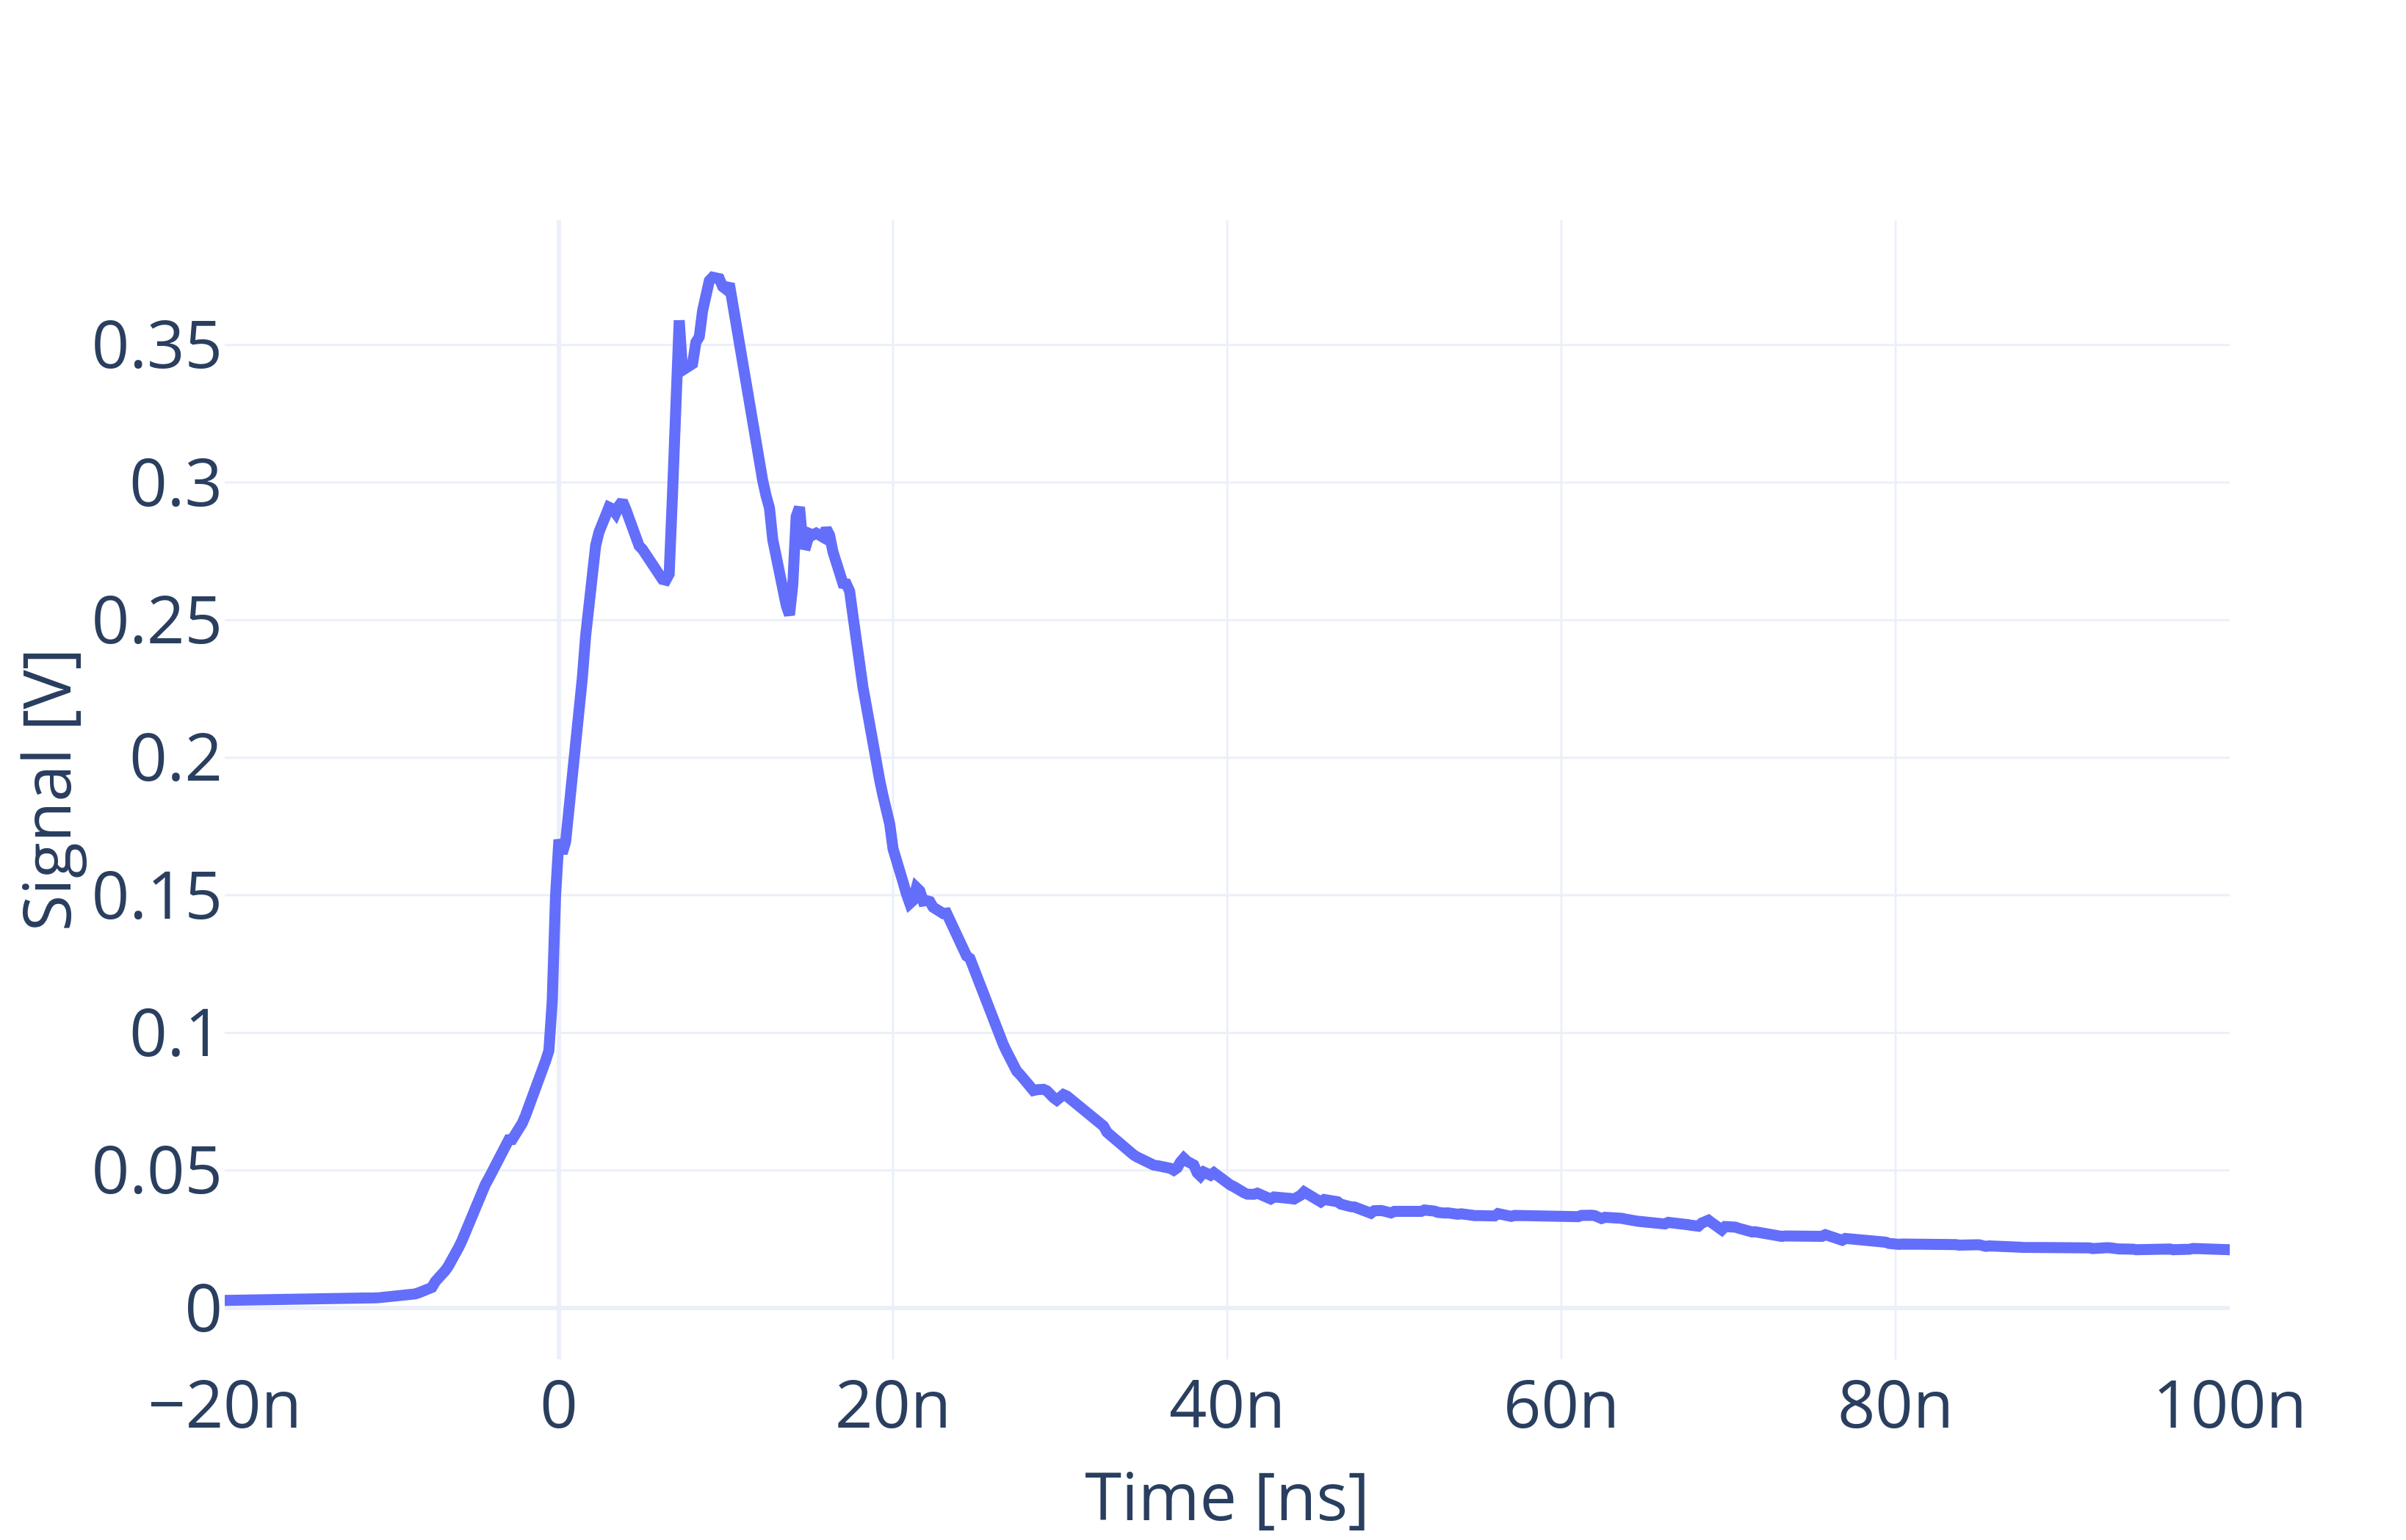
\includegraphics[width=0.27\textwidth,valign=c]{img/temporal_profile_new.png}
        \label{fig:profile}
        %\end{minipage}
        %\begin{minipage}{.4\textwidth}
        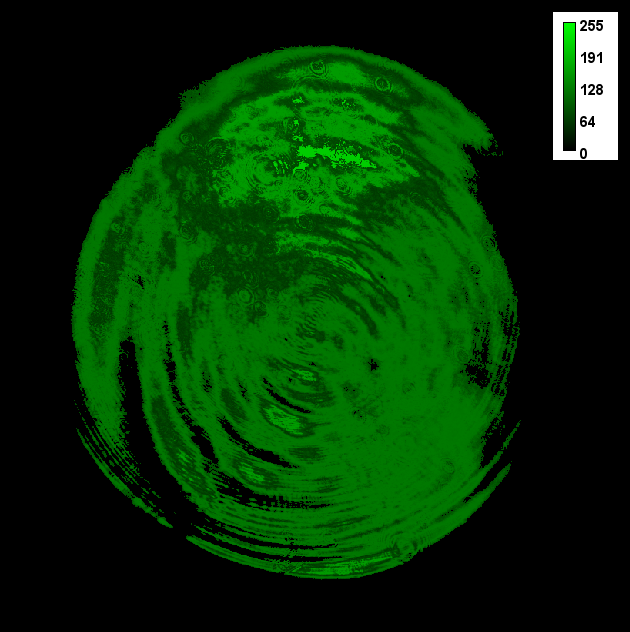
\includegraphics[width=0.15\textwidth,valign=c]{img/C2-v3_36_mJ_scale.png}
        \label{fig:profile}
        %\end{minipage}%

        \caption{Description of images from left to right: (1) Temporal shape of Litron system laser pulse (2) Near field camera profile of Litron system laser pulse}
        \label{fig:profile}
        \end{center}

        \end{figure}
    

    %%%%%%%%%%%%%%%%%%%%%%%%%%%%%%%%%%%%%%%%%%%%%%%%%%%%%%%%%%%%%%%%%
    %%%%%%%%%%%%%%%%%%%%%%%%%%%%%%%%%%%%%%%%%%%%%%%%%%%%%%%%%%%%%%%%%
    %%%%%%%%%%%%%%%%%%%%%%%%%%%%%%%%%%%%%%%%%%%%%%%%%%%%%%%%%%%%%%%%%


\subsection{Experimental setup}


\subsection{Acoustic emission}

An optical microphone is directly measuring the changes in the density of the optical medium. An optical microphone consists of a miniaturized Fabry-Pérot laser interferometer (FPI). The FPI comprises two semi-transmissive mirrors arranged at a distance matching a multiple of the laser’s half-wavelength $d$ and two lenses.

An incoming laser beam passes between the two mirrors multiple times. Part of the light in each pass is transmitted through the second surface. This process generates multiple reflected beams out of phase by a constant increment and forms interference fringes. The interference fringes form concentric circles when focused by a lens. The FPI multiple reflections follow the interference condition for thin films:

\begin{gather} \label{interference}
2d\cos\alpha = m\lambda
\end{gather} 

where:

\begin{itemize}

    \item $d$ -- distance between the two mirrors,
    \item $\alpha$ -- angle of incidence,
    \item $m$ -- order of the interference maximum,
    \item $\lambda$ -- laser wavelength.
    
\end{itemize}

Equation \ref{interference} represents the condition for the constructive interference intensity maximum \cite{fpi}.

 The optical microphone consists of two units:

\begin{itemize}
 
    \item the acoustic detection system, consisting of the optical sensor head and the driver unit comprising laser and detector,

    \item the analogue-to-digital converter with acquisition software \cite{fischer_rohringer_panzer_hecker_2017}.

\end{itemize}

 The principle of operation of the optical microphone is depicted in Figure \ref{fig:optical_microphone_principle}. The incoming sound signal causes small changes in the density of the optical medium between the two mirrors of the FPI. The FPI is inside the optical sensor head. These changes in density alter the optical index of refraction of the medium and, consequently, the laser’s propagation speed and wavelength. The distance between the two mirrors is fixed, so the change of the laser’s wavelength results in the change of the condition for the constructive interference intensity maximum, which changes the transmitted laser intensity. The laser intensity is measured with a photodiode and converted to an electrical signal.

 %% optical microphone principle 
\begin{figure}[h]
    \centering
    
\includegraphics[width=0.9\linewidth]{img/optical_microphone_principle.jpg}
    \caption{Principle of optical microphone -- the ultrasonic signal is detected optically by the change of the refractive index within a FPI etalon inside the optical sensor head \cite{fischer_rohringer_panzer_hecker_2017}}
    \label{fig:optical_microphone_principle}
\end{figure}

The Xarion Eta250 Ultra optical microphone is used. The main features of the Xarion Eta250 Ultra optical microphone are listed in Table \ref{tab:xarionparameters}~\cite{xarion_eta}. 

\begin{table}[h!] 
\centering
    \begin{threeparttable}
        \begin{tabular}{|c | c|} 
        \hline
            \textbf{Parameter} & \textbf{Value} \\ [0.5ex] 
        \hline
        Transducer type & Membrane-free, optical  \\ 
        \hline
            Frequency range &  10 Hz – 1 MHz \\
        \hline
            Dynamic range & 100 dB  \\
        \hline
            Self-noise, full bandwidth & 50 mPa  \\ 
        \hline
            Max. sound pressure for THD < 3 & 400 Pa \tnote{a} \\
        \hline
            Sensitivity & 10 mV/Pa @ 1 kHz  \\
        \hline
            Output impedance & 50 \Omega  \\
        \hline
            Polar pattern & Omnidirectional  \\
        \hline
        \end{tabular}
        \begin{tablenotes}
            \small
            \item[a] THD = Total Harmonic Distortion. 
        \end{tablenotes}
        
    \end{threeparttable}
        \caption{Xarion Eta250 Ultra optical microphone parameters \cite{xarion_eta}}
\label{tab:xarionparameters}
\end{table}
\input{sections/03theory.tex}
\section{Results and discussion} \label{sec:conclusions}
    \lipsum[6-7]
\section{Conclusion} \label{sec:conclusions}
    \lipsum[6-7]
\section*{Acknowledgements} \label{sec:acknowledgements}

This research was supported/partially supported by [Name of Foundation, Grant maker, Donor]. In addition, we thank our colleagues from [Name of the supporting institution] who provided insight and expertise that greatly assisted the research. However, they may not agree with all of the interpretations/conclusions of this paper.
We thank [Name Surname, title] for assistance with [particular technique, methodology], and [Name Surname, position, institution name] for comments that significantly improved the manuscript.
We would also like to show our gratitude to the (Name Surname, title, institution) for sharing their pearls of wisdom with us during the course of this research, and we thank 3 “anonymous” reviewers for their so-called insights. Finally, we are also immensely grateful to (List names and positions) for their comments on an earlier version of the manuscript, although any errors are our own and should not tarnish the reputations of these esteemed persons.
% \begin{thebibliography}{4}
\bibitem{Griffiths}
D. J. Griffiths,
\textit{Introduction to Electrodynamics}
(Cambridge University Press, Cambridge, 2017).

\bibitem{Fleming}
A. Bobrinha,
Revista Brasileira de Lorem Ipsum \textbf{23},
179 (2002).

\bibitem{Feynman}
R. P. Feynman, R. B. Leighton and M. Sands,
\textit{Lições de Física de Feynman}
(Editora Bookman, Porto Alegre, 2008).

\bibitem{Jackson-CE}
J. D. Jackson,
\textit{Classical Electrodynamics}
(John Wiley \& Sons, Danvers, 1999).

 %% acoustic wu
  @misc{wu_zhao_qiao_liu_zhang_hu_2018, title={Acoustic wave detection of laser shock Peening}, url={http://oejournal.org/article/doi/10.29026/oea.2018.180016},
  journal={Opto-Electronic Advances}, publisher={Opto-Electronic Advances},
  author={Wu, Jiajun and Zhao, Jibin and Qiao, Hongchao and Liu, Xuejun and Zhang, Yinuo and Hu, Taiyou}, 
  year={2018},
  month={Nov}
  
} 

\end{thebibliography}



\printbibliography

\appendix*
\section{Appendix} \label{sec:appendix}
    \lipsum[9-11]

\end{document}
